
\section{روش‌های یادگیری توزیع‌شده فدرالی}
یادگیری فدرال (\lr{FL})\footnote{\lr{Federated Learning}} به مدل‌های بصری (\lr{visual}) امکان می‌دهد تا با استفاده از داده‌های دنیای واقعی دستگاه‌های تلفن همراه با حفظ حریم خصوصی آموزش داده شوند. با توجه به ماهیت توزیع‌شده دستگاه‌ها و عملکرد کاربران آن‌ها، آمار داده‌ها در این دستگاه‌ها احتمالاً به طور قابل توجهی متفاوت است. در حالی که در آموزش مرکز داده\footnote{\lr{Data-center training}}، دسته‌های داده معمولاً می‌توانند \lr{IID} (مستقل و دارای توزیع یکسان) فرض شوند، اما این فرض در تنظیمات یادگیری فدرال بعید است. در چند سال گذشته، ابزارهای یادگیری فدرال برای پرداختن به آموزش‌های توزیع‌شده در مقیاس بزرگ در بسیاری از دستگاه‌ها یا گره‌ها، با قابلیت‌های حفظ حریم خصوصی در مقایسه با سیستم‌های یادگیری ماشین توزیع‌شده (\lr{DML})، استفاده شده‌اند. الگوریتم‌های یادگیری فدرالی به جای اشتراک‌گذاری داده‌های خام مانند یادگیری ماشین توزیع‌شده به تبادل نمونه‌های آموزش‌دیده محلی و پارامترهای یادگیری ماشین همچون وزن‌ها و بایاس‌های شبکه‌ عصبی متکی هستند. 

مساله بهینه‌سازی ضمنی در یادگیری فدرالی با عنوان بهینه‌سازی فدرالی  اشاره می‌شود. بهینه‌سازی فدرالی چندین ویژگی کلیدی دارد که آن را از یک مساله بهینه‌سازی توزیع‌شده معمول متمایز می‌کند. 
\begin{itemize}
	\item 
	\lr{Non-IID}: داده های آموزشی در یک کلاینت معین معمولاً بر اساس استفاده از دستگاه تلفن همراه توسط یک کاربر خاص است و از این رو مجموعه داده محلی هر کاربر خاص نماینده توزیع جمعیت نخواهد بود.
	\item 
	\lr{Unbalanced}: برخی از کاربران نسبت به سایرین از سرویس یا برنامه سنگین‌تری استفاده می‌کنند که منجر به مقادیر متفاوتی از داده‌های آموزشی محلی می شود.
	\item 
	\lr{Massively distributed}: انتظار  داریم تعداد کلایت‌هایی که در یک بهینه‌سازی شرکت می‌کنند بسیار بیشتر از میانگین تعداد نمونه‌های هر مشتری باشد.
	\item
	\lr{Limited communication}: دستگاه‌های تلفن همراه اغلب آفلاین یا دارای اتصالات کند و گران هستند.
\end{itemize}

کاربردهای عملی زیادی از ایده کلی یادگیری فدرال وجود دارد. دو تنظیمی که ممکن است به طور قابل توجهی بر طراحی الگوریتم‌های عملی تأثیر بگذارد به شرح زیر می‌باشند:
\begin{itemize}
	\item 
	یادگیری فدرالی بین دستگاهی یا \lr{Cross-device}: در این نوع، یادگیری ماشین با استفاده از جمعیت زیادی از دستگاه‌های موبایل مورد نظر است.
	\item 
	یادگیری فدرالی بین سازمانی یا \lr{Cross-silo}: در این نوع، یادگیری مشارکتی بین چندین سازمان مورد هدف است.
\end{itemize}

هر دو تنظیم دارای ناهمگنی داده‌ها، محاسبات و همچنین محدودیت‌های ارتباطی و حریم خصوصی هستند، اما تفاوت‌های ظریفی نیز دارند. تنظیمات بین دستگاهی و بین سازمانی عمدتاً توسط محدودیت‌های تحمیلی سیستم تعریف می‌شوند و تنها دو مورد از بسیاری از روش‌های ممکن یادگیری فدرال می‌باشند. این دو تنظیم به دلیل کاربرد زیاد و پذیرش عملی آنها توسط صنعت تا به امروز موضوع بسیاری از تحقیقات در مورد یادگیری فدرال بوده‌اند. دیگر سناریوهای یادگیری فدرال شامل شبکه‌هایی هستند که در آن‌ها ارتباطات بسیار مطمئن با تأخیر کم ضروری است. وسایل نقلیه در جاده، یا به طور کلی شبکه‌های لبه بی‌سیم نمونه‌ای از این شبکه‌ها می‌باشد. در ادامه تفاوت‌های این دو تنظیم مورد بررسی قرار گرفته‌اند.
\begin{itemize}
	\item 
	\textbf{تعداد کلاینت‌ها}: تعداد کل کلاینت‌ها در یادگیری فدرال بین دستگاهی معمولاً بسیار بیشتر از یادگیری فدرال بین سیلو است. تعداد کلاینت‌ها (سازمان‌ها) در یادگیری فدرال بین سیلو می‌تواند به اندازه دو، اغلب ده‌ها یا صدها باشد، در حالی که تعداد کلاینت‌ها‌ (دستگاه‌ها) در یادگیری فدرال بین دستگاهی می‌تواند به راحتی از میلیون‌ها دستگاه فراتر رود. مقدار داده‌های خصوصی در هر مشتری در یادگیری فدرال بین دستگاهی می‌تواند کمتر از یادگیری فدرال بین سیلو باشد. این ممکن است بر ناهمگنی داده‌ها تأثیر بگذارد.
	\item 
	\textbf{دردسترس بودن کلاینت‌ها}: کلاینت‌های بین سیلو معمولاً در مراکز داده نگهداری می‌شوند، که به معنای در دسترس بودن بالا است که احتمالاً همه مشتریان را قادر می‌سازد در هر دور شرکت کنند. در مقابل، جمعیت زیاد با در دسترسی متناوب در یادگیری فدرال بین دستگاهی نشان می‌دهد که سرور فقط می‌تواند از طریق برخی از فرآیندهای نمونه‌برداری به مشتریان دسترسی داشته باشد و سرور فقط توانایی محدودی برای کنترل آن دارد. در تنظیمات بین دستگاهی، در دسترس بودن مشتری برای شرکت در آموزش ممکن است با توزیع داده‌های آموزشی محلی آن نیز مرتبط باشد و تغییرات روزانه را معرفی کند که الگوریتم‌های بهینه‌سازی ممکن است به آن نیاز داشته باشند.
	\item 
	\textbf{توپولوژی اتصال}: اتصالات همتا به همتای مستقیم (غیر از سرور) معمولاً در پلتفرم‌های دستگاه موبایل به خوبی پشتیبانی نمی‌شوند، در حالی که در تنظیمات بین سیلو، چنین اتصالات مستقیم مشتری به مشتری ممکن است آسان‌تر باشد. در یادگیری فدرالی بین سیلو، محققان انواع الگوهای ارتباطی از قبیل یادگیری فدرالی غیرمتمرکز، یادگیری فدرالی افقی، یادگیری فدرالی سلسله‌مراتبی و یادگیری تقسیم‌شده را بررسی کرده‌اند.
	\item
	\textbf{محدودیت‌های ارتباطی و محاسباتی}: محدودیت‌های محاسباتی و ارتباطی در تنظیمات بین دستگاهی سخت‌تر هستند. دستگاه اغلب محاسبات و قدرت ارتباطی محدودی دارند، در حالی که کلاینت‌ها در تنظیمات بین سیلو اغلب می‌توانند مراکز داده‌ای باشند که قادر به استقرار شتاب‌دهنده‌های سخت‌افزاری و پیوندهای ارتباطی با پهنای باند بالا هستند.
	\item 
	\textbf{حالت محاسبات محلی-کلاینت}: با توجه به جمعیت زیاد، اهداف حفظ حریم خصوصی در سطح کلاینت و ضرورت نمونه‌گیری، در تنظیمات بین دستگاهی، ممعمولاً فرض می‌شود که دستگاه‌ها هیچ شناسه‌ای ندارند و ممکن است فقط یک بار در کل فرآیند آموزشی شرکت کنند. بنابراین، در این تنظیمات، الگوریتم‌های بدون \lr{client-side state} به طور کلی ضروری هستند. در مقابل، از آنجایی که اکثر مشتریان در اکثر دوره\textbf{}‌های آموزش بین سیلو شرکت می‌کنند، الگوریتم‌های \lr{stateful} مناسب هستند.
\end{itemize}

یادگیری فدرالی از لحاظ وجود یا عدم وجود یک سرور مرکزی در معماری شبکه مورد استفاده به دو دسته اصلی یادگیری فدرالی متمرکز و غیرمتمرکز تقسیم می‌شوند. در ادامه‌ی این بخش به طور مفصل روش‌های توزیع دادها، انواع یادگیری فدرالی و الگوریتم‌های آن‌ شرح داده می‌شوند.
\subsubsection{روش‌های توزیع‌ داده‌ها در یادگیری فدرال}
برای مطالعه بهینه‌سازی فدرال، باید نحوه توزیع داده‌ها بر روی کلاینت‌ها را مشخص کنیم. در مقاله \cite{Fed1} دو روش برای پارتیشن‌بندی داده‌های \lr{MNIST} روی کلاینت‌ها بررسی شده است: \lr{IID}، که در آن داده‌ها به‌هم ریخته می‌شوند، و سپس بین 100 مشتری تقسیم می‌شوند که هر کدام 600 نمونه دریافت می‌کنند، و \lr{Non-IID}، که در آن ابتدا داده‌ها را بر اساس برچسب رقمی مرتب می‌شوند، آن به 200 قسمت با اندازه 300 تقسیم می‌شوند. و به هر 100 کلاینت 2 زیرمجموعه اختصاص داده می‌شود. این یک پارتیشن‌بندی \lr{Non-IID} از داده‌ها است، زیرا اکثر کلاینت‌ها تنها نمونه‌هایی از دو رقم را خواهند داشت. بنابراین، می‌توان درجه شکست الگوریتم‌ها را در داده‌های \lr{Non-IID} بررسی کرد. به این روش حالت \lr{ sort-and-partition } گفته می‌شود. در \cite{Fed2} به طور مشابه پارتیشن‌های بسیار زیادی بر روی مجموعه داده \lr{CIFAR-10 } تولید کرده و جمعیتی متشکل از 10 کلاینت در مجموع تشکیل داده شده است. این تنظیمات تا حدودی غیر واقعی هستند، زیرا یادگیری فدرال عملی معمولاً شامل مجموعه بزرگتری از کلاینت‌ها با توزیع‌های پیچیده‌تر از پارتیشن‌بندی‌های ساده است. در برخی دیگر از مقالات توزیع داده‌های واقعی‌تر در کلاینت‌ها استفاده شده است. 

در مقاله \cite{Fed3} مجموعه داده \lr{EMNIST} با پارتیشن‌بندی بر روی نویسندگان ارقام به جای پارتیشن‌بندی ساده بر روی کلاس ارقام استفاده شده است. در مقاله \cite{Fed4} توزیع دریکله با پارامتر غلظت 0.5 برای ترکیب کردن مجموعه داده‌های غیریکسان استفاده می‌شود. به طور مشابه، مقاله \cite{Fed5} یک محدوده پیوسته از پارامتر غلظت در توزیع دریکله را با کاوش دقیق در تنظیمات بهینه‌سازی و هایپرپارامتر بهینه جستجو می‌کند. نویسندگان برای ترکیب جمعیتی از کلاینت‌های غیریکسان را از توزیع دیریکله ترسیم می‌کنند، که $p$ توزیع کلاس قبلی را روی $N$ کلاس مشخص می‌کند، و $α > 0$ پارامتر غلظتی است که یکسانی را در بین کلاینت‌ها کنترل می‌کند. زمانیکه $\alpha\to \inf$، تمام کلاینت‌ها دارای توزیع یکسانی با قبلی هستند و زمانیکه $\alpha\to 0$ هر کلاینت شامل نمونه‌هایی از یک کلاس است که به صورت تصادفی انتخاب شده‌اند.

\subsubsection{یادگیری فدرالی متمرکز}
یادگیری فدرال متمرکز یک الگوی یادگیری ماشین توزیع‌شده است که در آن تعداد زیادی از گره‌ها با یک سرور مرکزی هماهنگ می‌شوند تا یک مدل را بدون به اشتراک گذاشتن داده‌های آموزشی خود یاد بگیرند. در این الگوریتم‌ها داده‌های خام گره‌ها هرگز با سرور یا سایر گره‌ها به اشتراک گذاشته نمی‌شود. این امر یادگیری فدرال را از بهینه‌سازی توزیع‌شده سنتی متمایز می‌کند و نیاز به رقابت با داده‌های ناهمگن دارد. در مفهوم اساسی یادگیری فدرال، به دنبال کمینه‌سازی تابع هدف هستیم. تابع هدف یادگیری فدرالی در رابطه زیر آورده شده است. 

\begin{equation}\label{e115}
	\begin{cases}
		\min_{w\in R^d} f(w)=\frac{1}{P} \sum_{i=1}^{|p|}F_i(w)\\
		F(w)=E_{i\sim P}[F_i(w)], \qquad  where \quad F_i(w)=E_{\xi\sim D_i}[f_i(w,\xi)]
	\end{cases}
\end{equation}
که $w\in R^d$ پارامتر مدل عمومی را نشان می‌دهد و $F_i: R^d\to R$ تابع هدف محلی در گره $i$ است. $P$ یک توزیع روی جمعیت گره‌ها است. تابع خطا محلی در گره $i$ یعنی $f_i(w,\xi)$ اغلب برای تمام گره‌ها یکسان است اما توزیع داده محلی $D_i$ اغلب متفاوت خواهد بود. انواع الگوریتم یادگیری درالی متمرکز در ادامه شرح داده شده است.

\subsubsection{الگوریتم \lr{FedSGD}}
در الگوریتم یادگیری \lr{FedSGD} یک کسر $C$ از گره‌ها در هر دور انتخاب شده و گرادیان تابع خطا روی تمام داده‌های نگه‌داری شده توسط این گره‌ها محاسبه می‌شود. در واقع پارامتر $C$ اندازه دسته داده کلی را کنترل می‌کند. به صورتی که $C=1$ معادل گرادیان کاهشی \lr{full-batch} بدون حالت تصادفی (\lr{non-stochastic}) است. گرادیان‌های محاسبه شده به سرور مرکزی ارسال می‌شوند و سرور مرکزی گرادیان‌ها را تجمیع کرده و رابطه به‌روزرسانی زیر را بر روی مدل کلی اعمال می‌کند:
\begin{equation}\label{e116}
	w_{t+1}=w_t-\eta \sum_{k=1}^K \frac{n_k}{n}g_k
\end{equation}
که $K$ تعداد گره‌هایی را نشان می‌دهد که داده‌ها روی آنها پارتیشن‌بندی شده‌اند. با توجه به اینکه $P_k$ مجموعه اندیس داده‌ها بر روی گره $k$ را نشان می‌دهد، $n_k=|P_k|$ تعداد داده‌های موجود در گره $k$ و $n=\sum_{k\in K} n_k$ تعداد کل داده‌ها را نشان می‌دهند. 

\subsubsection{الگوریتم \lr{FedAvg}}
در الگوریتم یادگیری \lr{FedAvg} یک کسری از گره‌ها در هر دور انتخاب شده و هر گره انتخاب شده به صورت محلی یک گام از گرادیان کاهشی بر روی مدل جاری و با استفاده از داده‌های محلی خودش اجرا می‌کند. هنگامی که الگوریتم به این صورت نوشته شود، می‌توانیم با تکرار به‌روزرسانی محلی، محاسبات بیشتری به هر گره اضافه کنیم. 
\begin{equation}\label{e117}
	w_{t+1}^k=w_t-\eta g_k
\end{equation}
و سپس سرور مدل‌های محلی دریافت شده از گره‌ها را تجمیع کرده و با استفاده از رابطه \ref{e118} که یک میانگین وزن‌دار از مدل‌های نتیجه شده است، مدل عمومی را به‌روزرسانی می‌کند:
\begin{equation}\label{e118}
	w_{t+1}=\sum_{k=1}^K \frac{n_k}{n}w_{t+1}^k
\end{equation}

در مقاله \cite{Fed1} بر روی خصوصیات \lr{unbalanced} و \lr{Non-IID} تاکید شده است. یک طرح به‌روزرسانی همزمان که در دورهایی (\lr{round}) از ارتباطات پیش می‌رود. یک مجموعه ثابتی از \lr{K} گره با مجموعه داده‌های محلی ثابت خودشان وجود دارد. در ابتدای هر دور یک کسر تصادفی $C$ از گره‌ها انتخاب شده و سرور پارامترهای مدل جاری عمومی را برای گره‌های انتخاب شده ارسال می‌کند. هر گره انتخاب شده محاسبات محلی را بر اساس مدل عمومی و داده‌های محلی خودش اجرا می‌کند و سپس به‌روزرسانی‌ها به سرور ارسال می‌شوند. سرور این به‌روزرسانی‌ها را به مدل عمومی اعمال می‌کند و این فرآیند تا رسیدن به همگرایی مورد نظر ادامه می‌یابد. نویسندگان مقاله نشان می‌دهند که با استفاده از داده‌های \lr{MNIST} الگوریتم \lr{FedAvg} بر روی گره‌ها با توزیع غیریکسان داده‌ همچنان به دقت $\%99 $ همگرا می‌شود، اگرچه دور‌های بیشتری را نسبت به گره‌ها با توزیع یکسان داده انجام می‌دهد.

\subsubsection{الگوریتم \lr{FedAvgM}}
الگوریتم \lr{FedAvg} از \lr{vanilla SGD} در سرور استفاده می‌کند در حالی که الگوریتم \lr{FedAvgM} از \lr{SGD} با پارامتر تکانه $0.9$ بر روی سرور استفاده می‌کند. رابطه به‌روزرسانی در سرور مرکزی با استفاده از رابطه \ref{e119} انجام می‌شود \cite{Fed5}.

\begin{equation}\label{e119}
	\nu =\beta\nu+\Delta w,\qquad w=w-\nu
\end{equation}

\subsubsection{الگوریتم \lr{FedOPT}}
با فرض این‌که در دور $t$، سرور مرکزی مدل $w_t$ و مجموعه $K$ گره‌ دارد. $w_i^t $ مدل گره $i\in K$ بعد از یادگیری محلی است. رابطه به‌روزرسانی در \lr{FedAvg} به صورت زیر بازنویسی می‌شود:
\begin{equation}\label{e120}
	w_{t+1}=\frac{1}{K}\sum_{i\in K}w_i^t=w_t - \frac{1}{K}\sum_{i\in K}(w_t-w_i^t)
\end{equation}
فرض کنید 

\begin{equation}\label{e121}
	\Delta_i^t=w_i^t-w_t
\end{equation}
آنگاه خواهیم داشت
\begin{equation}\label{e122}
	\Delta_t=\frac{1}{K}\sum_{i\in K}\Delta_i^t
\end{equation}
با توجه به روابط ذکر شده فوق، به‌روزرسانی سرور در \lr{FedAvg} معادل به کار بردن \lr{SGD} با شبه‌-گرادیان $-\Delta_t$ با نرخ یادگیری $\eta=1$ است. البته انتخاب‌های دیگر برای $\eta$ نیز ممکن است. همچنین می‌توان از بهینه‌سازی‌هایی غیر از \lr{SGD} در گره‌ها استفاده کرد یا از یک قانون به‌روزرسانی جایگزین در سرور استفاده کرد. این الگوریتم‌ها، که در مجموع از آن به عنوان \lr{FedOPT} یاد می‌شود\cite{Fed6}.

\subsubsection{الگوریتم‌های \lr{FedADAGRAD}، \lr{FedYOGI} و \lr{FedADAM}}

در این دسته از الگوریتم‌ها از روش‌های بهینه‌سازی تطبیقی همچون \lr{ADAM}، \lr{ADAGRAD} و \lr{YOGI} در بهینه‌سازی سمت سرور و از الگوریتم \lr{SGD} در سمت کلاینت استفاده می‌شود. با استفاده از روش‌های بهینه‌سازی تطبیقی در سرور و الگوریتم \lr{SGD} در کلاینت‌ها، می توان اطمینان داشت که روش ما هزینه ارتباطی مشابه \lr{FedAvg} خواهد داشت و در تنظیمات بین دستگاهی کار می‌کند. پارامتر $\tau$ درجه تطبیق‌پذیری الگوریتم‌ها را کنترل می‌کند. مقادیر کوچکتر $\tau$ درجه تطبیق‌پذیری بالاتری را ارائه می‌دهند. با توجه به اینکه $\Delta_t=\sum_{i\in K}\frac{n_i}{n}\Delta_i^t$ و $m_t=\beta_1 m_{t-1}+(1-\beta_1)\Delta_t$ است، روابط به‌روزرساني الگوریتم‌های \lr{FedAdagrad}، \lr{FedYogi} و \lr{FedAdam} به صورت زیر می‌باشند:


\begin{equation}\label{e124}
	\begin{cases}
		\nu_t =\nu_{t-1}+\Delta_t^2 \quad (FedAdagrad)\\
		w_{t+1}=x_t+\eta\frac{m_t}{\sqrt{\nu_t}+\tau}
	\end{cases}
\end{equation}

\begin{equation}\label{e125}
	\begin{cases}
		\nu_t =\nu_{t-1}-(1-\beta_2)\Delta_t^2 sign(\nu_{t-1}-\Delta_t^2) \quad (FedYogi)\\
		w_{t+1}=x_t+\eta\frac{m_t}{\sqrt{\nu_t}+\tau}
	\end{cases}
\end{equation}

\begin{equation}\label{e126}
	\begin{cases}
		\nu_t =\beta_2\nu_{t-1}+(1-\beta_2)\Delta_t^2 \quad (FedAdam)\\
		w_{t+1}=x_t+\eta\frac{m_t}{\sqrt{\nu_t}+\tau}
	\end{cases}
\end{equation}

\subsubsection{یادگیری فدرالی غیرمتمرکز}
نسل بعدی سیستم‌های صنعتی مستقل و شبکه‌ای (یعنی ربات‌ها، وسایل نقلیه، هواپیماهای بدون سرنشین) پیشرفت‌هایی را در ارتباطات و محاسبات بسیار قابل اعتماد انجام داده‌اند. این سیستم‌های چند عاملی شبکه‌شده به یادگیری ماشین سریع، کارآمد و توزیع‌شده برای ارائه عملکرد بهتر نیاز دارند. مقاله \cite{Fed9} به بررسی فرصت‌های جدید یادگیری فدرالی برای سیستم‌های صنعتی شبکه‌ای نسل بعدی پرداخته شده است و مسائل باز با تمرکز بر رانندگی مشارکتی در وسایل نقلیه خودکار متصل و روباتیک مشارکتی در تولید هوشمند مورد بحث قرار گرفته است. راه‌حل‌های غیرمتمرکز یادگیری فدرالی پتانسیل بالایی برای نسل پنجم (\lr{5G}) صنعتی دارند. در فرآیندهای صنعتی خودکار، یادگیری فدرالی غیرمتمرکز اطلاعات را مستقیماً به ماشین‌های پایانی منتقل می‌کند که به عنوان عامل‌های مشارکتی هوشمند محسوب می‌شوند.

پیاده‌سازی‌های یادگیری فدرالی کاملاً توزیع‌شده بر روی شبکه‌های \lr{P2P} اجرا می‌شوند که با گراف‌های متصل دلخواه مشخص می‌شوند. یادگیری مشارکتی مبتنی بر \lr{SGD} غیرمتمرکز (\lr{DSGD}) است که همگرایی را تحت مفروضات تحدب قوی توابع خطا محلی و شبکه‌هایی با ماتریس مجاورت تصادفی مضاعف تضمین می‌کند. الگوریتم \lr{DSGD} مراحل \lr{SGD} روی دستگاه را برای به دست آوردن $w_k(t)$ با تبادل متقابل پارامترهای مدل برای هدایت همگرایی جایگزین می‌کند. تبادل متقابل با شایعات (\lr{gossip})، اجماع، یا الگوریتم‌های انتشار تنظیم می‌شود. 
در پیاده‌سازی \lr{gossip} یادگیری فدرال، در هر دور گره‌ه‌ها به صورت تصادفی یک همسایه از همسایگی انتخاب کرده و با تبادل مدل‌های محلی آنها را با میانگین‌گیری تطبیق می‌دهد. به دنبال آن \lr{SGD} بر روی داده‌های محلی اجرا می‌شود. یادگیری فدرال انتشاری مذاکرات گرادیان را پیاده‌سازی می‌کند. در هر دور گره‌ها مدل‌های محلی و گرادیان‌ها را با یک همسایه که دوباره به صورت تصادفی انتخاب شده است، مبادله می‌کنند. برای هر دو نوع پیاده‌سازی زمان صرف شده هر دور شامل انتقال پارامترهای یادگیری ماشین، تطبیق مدل و گام \lr{SGD} یا به‌روزرسانی است. به منظور محدود کردن سربار ارتباطی، پارامترهای مدل پراکنده یا کاهش می‌یابند. 
رویکردهای اولیه یادگیری فدرال بر اساس معماری کلاینت-سرور هستند، جایی‌که یک سرور پارامتر به عنوان دستگاه لبه برای هماهنگ کردن فرآیند یادگیری عمل می‌کند. از سوی دیگر، رویکردهای جدید یادگیری فدرال، معماری‌های مه را هدف قرار می‌دهند که در آن پارامترهای مدل به طور متقابل توسط دستگاه‌ها به اشتراک گذاشته می‌شوند و به روشی توزیع شده از طریق الگوریتم‌های اجماع  هماهنگ می‌شوند. این ابزارها به سرور پارامتر متکی نیستند، اما از پیوندهای \lr{V2X} (پیوندهای بین وسیله نقلیه و هر چیزی) با تاخیر کم بهره می‌برند. دستگاه‌ها از طریق شبکه‌های غیرمتمرکز، مش، یا دستگاه به دستگاه بدون تکیه بر سرور پارامتر همگام می‌شوند. سیاست‌های یادگیری فدرال به خوبی کاستی‌های مقیاس‌پذیری و حریم خصوصی را برطرف می‌کنند،در مقاله \cite{Fed11} با استفاده از اصول یادگیری فدرالی دو الگوریتم مبتنی بر اجماع به نام‌های \lr{CFA}\footnote{\lr{Consensus-based Federated Averaging}} و \lr{CFA-GE}\footnote{\lr{Consensus-based Federated Averaging-with Gradients Exchange}} برای شبکه‌های بسیار متراکم و کاملاً غیرمتمرکز بدون نیاز به یک سرور مرکزی برای هماهنگی فرآیند یادگیری با تمرکز بر مجموعه داده‌های تجربی جمع‌آوری شده در یک محیط صنعتی اینترنت اشیا پیشنهاد شده است. 

\subsubsection{الگوریتم \lr{CFA}}
الگوریتم \lr{CFA} توسعه‌ای از یادگیری فدرالی متمرکز است . بعد از مقداردهی اولیه $W_{0,k}$ در زمان $t=0$، در هر دور ارتباطی $t>0$ وسیله یا گره $k$ مدل به‌روزشده‌اش را ارسال و وزن‌های همسایه‌ها $w_{t,i},i\in N_k$ را دریافت می‌کند. بر اساس داده دریافت شده دستگاه مدل خود را به صورت متوالی به‌روزرسانی می‌کند تا مدل تجمیع‌شده حاصل گردد:
\begin{equation}\label{e127}
	\phi_{t,k}=w_{t,k}+\epsilon_t\sum_{i\in N_k}\alpha_{k,i}(w_{t,i}-w_{t,k})
\end{equation}
که $\epsilon_t$ اندازه گام و $\alpha_{k,i}$ وزن‌های ترکیب مدل‌ها هستند. سپس به‌روزرسانی گرادیان با استفاده از مدل تجمیع‌شده $\phi_{t,k}$  با اجرای \lr{ُSGD} بر روی تعدادی دسته از اندازه \lr{B} اجرا می‌شود.
\begin{equation}\label{e128}
	w_{t+1,k}=\phi_{t,k}-\eta_t \nabla L_{t,k}(\phi_{t,k})
\end{equation}

\subsubsection{الگوریتم \lr{CFA-GE}}
در الگوریتم \lr{CFA-GE} تبادل مشترک گرادیان‌های محلی و به‌روزرسانی مدل با پیروی از روش تکراری چهار مرحله‌ای نشان داده شده در شکل \ref{Pic33} انجام می‌شود. 
\begin{figure}[h]
	\begin{center}
		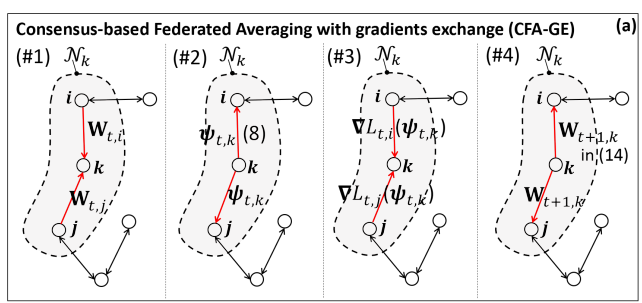
\includegraphics[scale=0.55]{Pic33.png}
		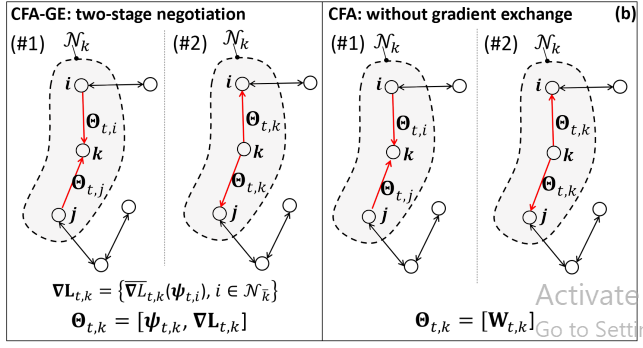
\includegraphics[scale=0.55]{Pic35.png}
		\caption{مراحل تبادل گرادیان‌ها و به‌روزرسانی مدل در الگوریتم \lr{CFA-GE}\cite{Fed11}}
		\label{Pic33}
	\end{center}
\end{figure}

مرحله اول آن مشابه الگوریتم \lr{CFA} است و $\phi_{t,k}$ را با تجمیع مدل مبتنی بر اجماع بدست می‌آورد. قبل از استفاده از $\phi_{t,k}$ برای به‌روزرسانی مدل محلی، به همان همسایگان بازخورد داده می‌شود (مرحله "مذاکره" یا \lr{negotiation} در مرحله 2 شکل \ref{Pic33}). سپس مدل $\phi_{t,k}$ توسط همسایگان برای محاسبه گرادیان‌ها با استفاده از داده‌های محلی آنها استفاده می‌شود. توجه داشته باشید که همه گرادیان‌ها بر روی یک دسته (یا مینی دسته) از داده‌های محلی محاسبه می‌شوند، در حالی که دسته/مینی‌دسته انتخابی می‌تواند در دورهای ارتباطی متوالی تغییر کند. گرادیان‌ها به دستگاه $k$ در مرحله 3 برمی‌گردند. در مقایسه با \lr{CFA}، این مرحله به هر دستگاهی اجازه می‌دهد تا با استفاده از داده‌های همسایه از گرادیان‌های اضافی بهره‌برداری کند و یادگیری را بسیار سریع‌تر می‌کند. بنابراین در دستگاه $k$، مدل محلی با استفاده از گرادیان‌های دریافتی $\nabla L_{t,k}(\phi_{t,k})$ مطابق رابطه \ref{e129} به‌روزرسانی می‌شود.

\begin{equation}\label{e129}
	\phi_{t,k}=\phi_{t,k}-\eta_t \sum_{i\in N_k}\beta_{k,i}P_{\Theta}[\nabla L_{t,i}(\phi_{t,k})]
\end{equation}
که $\beta_{k,i}$ وزن‌های ترکیب برای گرادیان‌ها هستند. در نهایت، همانطور که برای \lr{CFA} انجام شد.، به‌روزرسانی گرادیان با استفاده از مدل تجمیع‌شده $\phi_{t,k}$ و دسته دادهای محلی انجام می‌شود.

\begin{equation}\label{e130}
	w_{t+1,k}=\phi_{t,k}-\eta_t \nabla L_{t,k}(\phi_{t,k})
\end{equation}
برخلاف \lr{CFA}، \lr{، CFA-GE} نیاز دارد از پهنای باند و دورهای ارتباطی بیشتر برای تبادل همزمان گرادیان‌ها استفاده کند. به طور خاص، به استفاده فشرده‌تر از پیوندهای بی‌سیم \lr{D2D} برای به اشتراک‌گذاری مدل‌ها ابتدا در طول مذاکرات (مرحله شماره 2) و سپس ارسال گرادیان‌ها (مرحله 3) نیاز دارد. علاوه‌براین، هر دستگاه باید قبل از اعمال هر به‌روزرسانی مدل منتظر شیب‌های همسایه باشد. پیاده‌سازی دو مرحله‌ای \lr{CFA-GE}، اجرای روش مذاکره را برای بهبود زمان همگرایی (و تأخیر) ساده می‌کند. به عبارتی، هر دستگاه می‌تواند به‌روزرسانی‌ها را بدون انتظار برای پاسخ از همسایگان انجام دهد. با یک تعمیم ساده، دستگاه \lr{k} پارامترها را با همسایگان در دوره $t$ به صورت زیر مبادله می‌کند:
\begin{equation}\label{e130}
	\Theta_{t,k}=[\Phi_{t,k},\nabla L_{t,k}], \qquad  \nabla L_{t,k}:=\{\overline{\nabla L}_{t,k}(\phi_{t-1,i}),\forall i\in N_k\}	
\end{equation}

در راستای تکنیک‌های مبتنی بر تکانه، برای پیش‌بینی‌های $\bar{\nabla L_{t,k}}$ از میانگین متحرک وزن‌دار نمایی چند متغیره گرادیان‌های گذشته استفاده می‌شود.
\begin{equation}\label{e131}
	\overline{\nabla L}_{t,k}(\phi_{t-1,i})=\varrho \nabla L_{t,k}(\phi_{t-1,i})+(1-\varrho)\overline{\nabla L}_{t-1,i}
\end{equation}

با فرض اینکه وسیله $k$ قادر باشد پیام‌های $\Theta_{t,i}=[\Psi_{t,i},\nabla L_{t,i}]$  
را از همسایگان در هر دور $t$ دریافت کند، گام تجمیع مدل و گام به‌روزرسانی مدل با استفاده از گرادیان‌های دریافتی به صورت زیر است:

\begin{equation}\label{e132}
	\phi_{t,k}=w_{t,k}+\epsilon_t \sum_{i\in N_k}\alpha_{k,i}(\phi_{t,i}-w_{t,k})
\end{equation}

\begin{equation}\label{e133}
	\overline{\phi}_{t,k}=\phi_{t,k}-\eta_t \sum_{i\in N_k}\beta_{k,i}P_\Theta[\overline{\nabla L}_{t,i}(\phi_{t-1,k})]
\end{equation}


در مقاله \cite{Fed7} رویکرد یادگیری غیرمتمرکز فدرال به نام \lr{C-FL}\footnote{\lr{Consensus-driven FL}} برای وسایل نقلیه خودکار متصل به منظور دسته‌بندی عوامل جاده ارائه شده است. عوامل جاده مانند عابران پیاده، مخروط‌های ترافیکی، موانع، دوچرخه‌ها، اتومبیل‌ها و اتوبوس‌ها  که هر وسیله نقلیه آن‌ها را با اسکن محیط از طریق خود توسط سنسور \lr{Lidar} شناسایی می‌کند. نویسندگان یک روش سنجش مشارکتی را پیشنهاد کرده‌اند که در آن هدف وسایل نقلیه یادگیری مشارکتی یک مدل یادگیری ماشین عمیق مبتنی بر \lr{PointNet} برای استنباط نوع واقعی عوامل جاده با استفاده از ابرهای \lr{Lidar point } است. 

وسایل نقلیه مدل‌های محلی را با همسایگان‌شان از طریق اجماع میانگین ترکیب می‌کنند. سپس مدل‌های ترکیب شده با اجرای یک بهینه‌ساز روی داده‌های محلی خود به‌روزرسانی می‌کنند. فرایند یادگیری فدرال به طور کلی برای تعدادی دور ارتباطی اجرا می‌شود تا زمانی‌که یک اجماع حاصل گردد. در یادگیری فدرال پارامتر $w$ با اعمال یک روش کمینه‌سازی روی مجموع محدودی از توابع هدف یاد گرفته می‌شود.

\begin{equation}\label{e134}
	\hat{W}=\argminA_w L(w)=\argminA_w \sum_{i=1}^{N_\nu} \rho_i L_i(W)
\end{equation}
که $E_i=|\varepsilon_i|, \forall i\in\nu$ و $E=|\varepsilon|$ به ترتیب تعداد نمونه‌هاي وسیله نقلیه $i$ و تعداد کل نمونه‌های در دسترس است. $\rho_i=\frac{E_i}{E}$ است و $L_i(W)$ تابع خطا محلی وسیله نقلیه $i$ و $l(x_h,y_h;W)$ خطا محاسبه شده بر روی نمونه $(x_h,y_h)$ در حضور پارامترهای $W$ است. 
\begin{equation}\label{e135}
	L_i(w)=\frac{1}{E_i}\sum_{h=1}^{E_i}l(x_h,y_h;W)
\end{equation}
الگوریتم \lr{C-FL} یک زیرمجموعه بهینه‌سازی شده $W_{t,i}$ از لایه‌های مدل $Q<=N$ را هدف قرار می‌دهد، در حالیکه بقیه $N-Q$ فقط با استفاده از دادهای محلی و بهینه‌ساز انتخاب شده یادگرفته می‌شوند. برای $Q$ لایه پارامترهای مدل $W_{t,i}^{(Q)}$ بر روی هر دور ارتباطی تبادل می‌شوند. باقی لایه‌ها با استفاده از تنها داده‌های محلی یادگرفته می‌شوند و به صورت  $W_{t,i}^{(P)}=\{w_n^T,b_n\}_{n=1}^{N_Q-1}$ جمع آوری شده‌اند.

\begin{equation}\label{e136}
	W_{t,i}^{(Q)}=[w_{N-Q}^T,b_{N-Q},...,w_N^T,b_N]
\end{equation}

در هر دور ارتباطی وسیله نقلیه $i$ پارامترهای $Q$ لایه انتخاب شده و دریافت شده از همسایگانش  $j\in \nu_{t,i}$ را از طریق اجماع میانگین به‌روز می‌کند.
\begin{equation}\label{e136}
	\phi_{t,i}^{(Q)}=\sigma_{i,i}W_{t,i}^{(Q)}+\sum_{j\in \nu_{t,i}}\sigma_{i,j}W_{t,j}^{(Q)}
\end{equation}
که $\sigma_{i,j}$ وزن‌هایترکیب برای مدل‌های دریافت شده هستند و به صورت زیر مقداردهی می‌شوند:
\begin{equation}\label{e137}
	\sigma_{i,j}=\frac{E_j}{\sum_{j\in \nu_{t,i}}E_j},\qquad \sigma_{i,i}=\frac{E_i}{\sum_{j\in \nu_{t,i}}E_j}
\end{equation}

به محض کامل شدن فرایند اجماع، وسیله نقلیه $i$ پارامترهای اشتراکی $\phi_{t,i}^{(Q)} $ با $W_{t,i}^{(P)} $ را به صورت $\phi_{t,i}=[W_{t,i}^{(P)}, phi_{t,i}^{(Q)}]$ ترکیب کرده و بهینه‌ساز محلی را برای کمینه‌سازی خطای محلی $L_i(\phi_{t,i}^{(Q)})$ اجرا می‌کند. بهینه‌ساز \lr{Adam} به عنوان گزینه ترجیحی برای معماری‌های مبتنی بر \lr{PointNet} در نظر گرفته می‌شود که
\begin{equation}\label{e138}
	W_{t+1,i}=\phi_{t,i}-\Delta \phi_{t,i}
\end{equation}

\begin{equation}\label{e139}
	\begin{cases}
		\Delta\phi_{t,i}=\eta_t\frac{\sqrt{1-\beta_2^T}}{1-\beta_1^t}\frac{m_{t+1,i}}{\sqrt{\nu_{t+1,i}}+\delta}\\
		m_{t+1,i}=\beta_1 m_{t,i}+(1-\beta_1)\nabla L_{t,i}(\phi_{t,i})\\
		\nu_{t+1,i}=\beta_2\nu_{t,i}+(1-\beta_2)\nabla^2 L_{t,i}(\phi_{t,i})
	\end{cases}
\end{equation}

که $m_{t+1,i}$ و $\nu_{t+1,i}$ تخمین‌های تکانه اول و دوم گرادیان‌های $\nabla L_{t,i}(\phi_{t,i})$ در دور $t+1$ هستند. پارامترهای جدید محاسبه شده $W_{t+1,i}$ به همسایگان وسیله نقلیه $i$ ارسال شده و دور جدید آغاز می‌شود. این فرایند تا زمانی‌که پارامترهای مدل به مقدار خطای موردنظر همگرا شوند، ادامه می‌یابد. 